\documentclass{standalone}
\usepackage{tikz}
\usepackage{ctex,siunitx}
\usepackage{tkz-euclide}
\usepackage{amsmath}
\usetikzlibrary{patterns, calc}
\usetikzlibrary {decorations.pathmorphing, decorations.pathreplacing, decorations.shapes,}
\begin{document}
\small
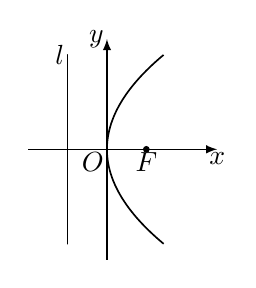
\begin{tikzpicture}[>=latex,scale=2.0,inner sep=1pt]
  \draw[thin,->](-0.5,0)--(0.7,0)node[below]{$x$};
  \draw[thin,->](0,-0.7)--(0,0.7)node[left]{$y$};
  \tkzDefPoints{0/0/O,0.25/0/F,-0.25/0/K,-0.25/0.5/P}
  \draw[semithick,domain=-0.6:0.6,samples=200] plot ({\x*\x},{\x});
  \tkzDrawPoints[fill=black](F)
  \tkzLabelPoints[below](F)
  \tkzDrawLine[semithick,add=0.2 and 1.2](P,K)
  \tkzLabelLine[pos=-0.2,left](P,K){$l$}
  \tkzLabelPoints[below left](O)
\end{tikzpicture}
\end{document}